\documentclass[10pt, a4paper]{article}
\usepackage[utf8]{inputenc}
 
\usepackage[danish]{babel}
\usepackage{blindtext}
\usepackage[hidelinks]{hyperref}
\usepackage{graphicx}
\usepackage{caption}
\usepackage{subcaption}
\usepackage{xcolor}
\usepackage{url}
% \usepackage[margin=1in]{geometry}
\usepackage[square,comma,numbers]{natbib}
\usepackage{float}
\usepackage{multicol}
% \usepackage[table,xcdraw]{xcolor}
\usepackage{color}
\usepackage{colortbl}
\usepackage{multirow}

\title{\textbf{EXO-AIDER}}
\author{Jacob Nørgaard}
 
\begin{document}

\pagenumbering{Alph}
\begin{titlepage}
\clearpage\maketitle
\thispagestyle{empty}
\end{titlepage}
\pagenumbering{arabic}

\section{Ideen bag projektet}
Ideen bag EXO-AIDER er at fremstille et let og kompakt overkrops exoskelet med torque nok til at assistere kørestolsbrugere fra siddende til stående possition. Exoskelettet vil være modulært som inkluderer albue og skulder ledene. 

En prototype til albueledet er fremstillet og aktuatoren er mindske i størrelse siden første revision som ses på \autoref{fig:first_rev_aktuator} og \autoref{fig:smaller_aktuator} hvor vægten også er mindsket fra 1 kg til 0.6 kg.


 \begin{figure}[htbp]
     \centering
     \begin{subfigure}[b]{0.3\textwidth}
         \centering
         \includegraphics[width=\textwidth]{figures/aktuater_minimeres1}
 		\caption{Version 1.0}
 		\label{fig:first_rev_aktuator}
     \end{subfigure}
     \hspace{1in}
     \begin{subfigure}[b]{0.3\textwidth}
         \centering
         \includegraphics[width=\textwidth]{figures/aktuater_minimeres2}
 		\caption{Version 2.1}
 		\label{fig:smaller_aktuator}
     \end{subfigure}
     \caption{Akuator vægt of størrelses reduktion}
\end{figure}

For at få en transparant oplevelse med exoskelettet er det vigtigt aktuatoren reagerer i forhold til brugerens intentioner. Dette gøres ved at have et sammenspil mellem mekanik, interaktions kontrol, sensorerer og brugeren, \autoref{fig:exo_interaction}.  

\begin{figure}[htbp]
	\centering
	\includegraphics[width=0.5\textwidth]{figures/human_interaction}
	\caption{Sammenspil mellem exoskelettet og brugeren}
	\label{fig:exo_interaction}
\end{figure}

De forskellige sensorerer i \autoref{fig:exo_interaction} der er i tankerne er force sensitive resistors (FSR) som måler hvor hårdt der trykkes og surface electromyography sensorer (sEMG) som måler de elektriske impulser i musklerne. Til montering af disse sensorer er der fremstillet et armbånd der kan sættes på brugeren arm og dermed have direkte kontakt til huden hvilket specielt er vigtig når der skal måles sEMG men er også generelt en god ide for at undgå interferens fra tøj osv.

Et armbånd med monterede købte sEMG sensorer er lavet og har vist lovende resultater. Armbåndet og dataen udvundet dermed har også været anvendt til at træne et support vector machine (SVM) netværk. Der er desuden blevet trænet et netværk på en person og efterfølgende er dette netværk testet på en anden person med gode resultater. Der har dog været problemer med de købe sEMG sensorer og det er derfor besluttet selv at fremstille disse sensorer med tilhørende hardware og software. 

Det endelige armbånd skal inkludere både sEMG og FSR sensorer og sammenkoblingen mellem de to typer signaler skal give et bedre indblik i brugerens intension til både at initiere bevægelse i exoskelettet men forhåbentligt også give en ide momentet.

\section{Afgrænsning af projektet}
Da projektet ikke strækker sig længere end et år frem fra nu er der blev lavet nogle afgrænsninger da det ikke er realistisk at nå i mål med et komplet exoskelet. I stedet for at ende med et exoskelet vil der blive fokuseret på at fremstille et armbånd med sEMG og FSR sensorer der kan kan måle musklernes aktivitet og derefter efterbehandle denne data ud fra det give et pålideligt resultat af brugerens aktivitet. Denne data vil senere kunne bruges i samarbejde med et exoskelet og give brugeren en transparant oplevelse ved brug. Armbåndet vil også kunne bruges i forbindelse med andre projekter hvor det vil være relevant at studere muskelaktiviteten.

Eftersom min opgave i dette projekt ikke er indenfor den mekaniske del af exoskelettet vil udgangspunktet derfor være at fokusere på armbåndet og arbejde med at koble begge typer signaler (sEMG og FSR) sammen til et funktionelt armbånd der giver et detaljeret indblik i muskelaktiviteten. Status på projektet og planen fra nu vil være baseret udelukkende på dette

\section{Status på projektet}
Status på projektet nu er baseret på hvad jeg har fået overleveret fra Simon og ændring til eksisterende løsninger kommer i næste afsnit. Afsnittene vil være delt op i hardware og software sektioner.

\subsection{Hardware}

Der er lavet et PCB med ADC, DAC'er med indgange til sEMG, FSR og IMU samt connections til ESP32 som ses på \autoref{fig:header_connector}.

\begin{figure}[htbp]
	\centering
	\includegraphics[width=0.8\textwidth]{figures/Pin_header_connector}
	\caption{Pin connections (ADC, DAC)}
	\label{fig:header_connector}
\end{figure}

Der er lavet en differensforstærker som kan kobles direkte på armbåndet (med kort ledning for at undgå støj). Forstærkeren kan kobles til et PCB der består af diverse filtre der giver et fokusområde fra 20 Hz til 500 Hz og med et notch filter ved 50 Hz for at mindske støj fra elnettet da denne type støj kan have stor indflydelse da 50 Hz ligger meget centralt i fokusområdet. Filter PCBet er derefter koblet til en ADC på førnævnte PCB som derefter kan kommunikere med microcontrolleren. 

Et blokdiagram der viser en oversigt over hele hardware blokken kan ses på \autoref{fig:hardware_block}.

\begin{figure}[htbp]
	\centering
	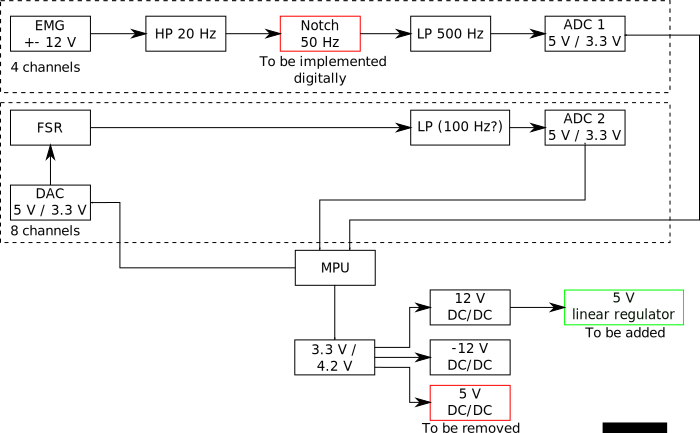
\includegraphics[scale=0.6]{../../Pictures/hardware_block_diagram.pdf}
	\caption{Hardware blockdiagram}
	\label{fig:hardware_block}
\end{figure}

\subsection{Software}

Software delen er splittet op i to dele, en Matlab del og en C++ del. Indtil videre har jeg størst indblik i Matlab koden som har et flow der ses på \autoref{fig:matlab_block}. 

\begin{figure}[H]
	\centering
	\includegraphics[scale=0.6]{../../Pictures/matlab_block_diagram.pdf}
	\caption{Matlab blockdiagram}
	\label{fig:matlab_block}
\end{figure}

Matlab kodens formål er at oprette forbindelse til microcontrolleren via Bluetooth og indsamle data fra diverse sensorer (FST, sEMG, IMU). Når dataen er indsamlet giver scriptet mulighed for at visualisere og efterprocessere dataen.

C++ koden der kører på microcontrolleren, og microcontrollerens opgave generelt, er at opsamle data fra sensorerne og sende det via Bluetooth. Når der er oprettet forbindelse mellem microcontrolleren og Matlab kan man vælge hvilke sensorer man vil samle data fra, eller om man vil samle data fra alle. Når man sender signal om dette valg tilbage til microcontrolleren, vælger koden hvilke ADCer der skal læses fra og sender denne data tilbage til Matlab.  

\section{Hvad er planen fra nu}
Planen fra nu består umiddelbart i at få en forståelse for hele systemet i detaljer og at rette fejl og mangler samt lave forbedring som er gennemgået med og overdraget fra Simon. 

En liste over ikke prioriteret opgaver og problematiker ses herunder.

\subsection{Hardware}

\begin{itemize}
	\item Der kommer intet signal gennem sEMG analog board. Det skal debugges.
	\begin{itemize}
		\item Muligvis en fejl i differensforstærkeren på boardet
	\end{itemize}
	\item Fjern hardware notch filter da det er meget følsom overfor komponent tolerancer og implementer digitalt
	\item Hardware low/high pass filtre skal have andre komponentværdier som kan ses i Simons Spice simulering
	\item Stort effektforbrug ved opstart af digitalt (ADC, DAC) board hvilket kan give problemer ved brug af lab forsyning
	\item Der skal kigges på design regler for SPI for muligvis at hæbe clock hastigheden
	\item Muligvis tilføje pull-down modstande til sEMG channels, de svæver ved ca 2V
	\item FSR og sEMG kan implementeres på samme PCB og fjerne FSR fra det digitale PCB
	\item Fjern 5V DC/DC supply, brug 5V linear regulator på 12 V forsyning i stedet som ses på \autoref{fig:hardware_block} 
\end{itemize}


\subsection{Software}

\begin{itemize}
	\item Software skal med sikkerhed køre 1 kHz. Dette skal testes igen da der kan være problemer med funktionen der er brugt til at teste.
	\item Bluetooth rate kan mindskes med en fakor 2 hvis ADC data sendes direkte i stedet for at konvertere det til float.
\end{itemize}

\section{Hvad er det endelige mål}

Det endelige mål er at få fremstillet et armbånd med tilhørende hardware og software der kan give et klar indblik i brugerens intention ved at analysere muskelaktiviteten med forskellige typer sensorer. Dette skal kunne bruges til implementering i et simpelt exoskelet der føles transparant for brugeren.


\bibliographystyle{ieeetr}%
% \bibliography{bib}

\end{document}